%% Phase III report -- CSCE 3602 / DSCI 3415 Fundamentals of Machine Learning
%% AI was used to help write this report and its code; the authors reviewed and edited every part (Section 11).
%% Red X = a number the remaining runs will fill in. Red [brackets] = a note for the authors, removed before submission.
\documentclass[sigconf,nonacm,10pt]{acmart}
\usepackage{tabularx}
\usepackage{booktabs}
\usepackage{multirow}
\sloppy
\settopmatter{printacmref=false}
\setcopyright{none}
\renewcommand\footnotetextcopyrightpermission[1]{}
\pagestyle{plain}

\newcommand{\X}{\textcolor{red}{\textbf{X}}}
\newcommand{\pending}[1]{\textcolor{red}{[#1]}}
\newcolumntype{Y}{>{\raggedright\arraybackslash}X}
\newcolumntype{L}[1]{>{\raggedright\arraybackslash}p{#1}}

\begin{document}

\title{Fair Price in a Moving Market: Predicting Residential Prices}
\subtitle{Phase III: Pilot Study of the Supervised Models}

\author{Zeyad Khaled}
\affiliation{%
  \institution{The American University in Cairo}
  \city{Cairo}
  \country{Egypt}}

\author{Mohamed Elsayed}
\affiliation{%
  \institution{The American University in Cairo}
  \city{Cairo}
  \country{Egypt}}

\begin{abstract}
We compare the supervised models covered in the course on the Zillow property file for Los Angeles, Orange and Ventura counties, predicting the natural log of each home's 2016 assessed value. Before training anything we rebuilt the dataset to answer the Phase 1 and Phase 2 feedback, and Section~\ref{sec:feedback} maps each comment to the change it caused. The rebuilt table holds 2,859,302 homes described by 17 features, which expand to 606 model columns. Every model followed one protocol: a five-fold search for its settings on 2,287,442 training homes, one final fit on all of them, and a single score on 571,860 test homes that played no part in any choice. The regression models were also scored as five-band price classifiers, next to seven classifiers trained on the bands: logistic regression, the perceptron, naive Bayes, and the forms the slides teach for K-nearest neighbours, the support vector machine, the mixture of experts and the Bayesian network. The Bayesian network placed the most homes in the right band (42.6\%). On the test homes the neural network reached $R^2 = 0.467$ on the log value with a median miss of 32.5\%, against 0.436 and 33.8\% for linear regression. Ranked on validation, the three strongest models were the neural network, the random forest and K-nearest neighbours. Averaging those three by voting did not beat the network alone (0.3731 against 0.3725 on the log scale). We choose the neural network.
\end{abstract}

\keywords{model comparison, cross-validation, regression, classification, property valuation}

\maketitle

%% ---------------------------------------------------------------------------------------------------------------
\section{Response to the Phase 1 and Phase 2 Feedback}
\label{sec:feedback}

Both earlier phases lost marks, and every comment pointed at something real. We rebuilt the dataset from the raw file before running a single model, so that the comparison in this report rests on data we can defend. Table~\ref{tab:feedback} pairs each comment with what we changed and the measurement behind the change. Appendix~\ref{app:fixes} lists all twelve fixes in full.

\begin{table*}[t]
\caption{Each comment from the first two phases, what changed, and the number that supports the change. Association values are measured on training homes (Section~\ref{sec:checks}).}
\label{tab:feedback}
\small
\renewcommand{\arraystretch}{1.2}
\begin{tabularx}{\textwidth}{@{}L{3.6cm}YY@{}}
\toprule
Comment (phase) & What we changed & Evidence \\
\midrule
Dataset too small; limits of the data not discussed (Phase 1) & The project moved to the Zillow file in Phase 2. This report states the limits of its label in Section~\ref{sec:limits}. & 2,985,217 parcels in the raw file; 2,859,302 homes kept. \\
What is FIPS? (Phase 2) & FIPS is the Federal Information Processing Standard county code. It is now read as a county name (6037 Los Angeles, 6059 Orange, 6111 Ventura). Its copy \texttt{regionidcounty} was removed with a measured reason. & Cram\'er's V of 1.000 between the two columns. The county itself was later dropped at 0.998 with the county land-use code. \\
Raw latitude and longitude used as inputs (Phase 2) & Coordinates became miles north and east of the median training home, since a degree of longitude here is 57 miles and a degree of latitude 69. Both were then dropped by the pair rule because ZIP code carries the same information. & 0.983 and 0.988 with ZIP code; ZIP code is 0.490 with the label against 0.119 and 0.013. \\
City, county and region dropped (Phase 2) & All five location columns were brought back and measured. ZIP code, neighbourhood and census tract are kept as one-hot groups. City and county were dropped by the measured pair rule, not by assumption. & 325, 98 and 16 model columns. City is 0.921 with ZIP code and weaker with the label (0.391 against 0.490). \\
No distribution analysis; log taken with no analysis (Phase 2) & Figure~\ref{fig:distributions} shows the label and the living area before and after the log, with the skew of each. & Label skew 18.9 falls to $-0.12$; living-area skew 262.1 falls to 0.39. \\
A decision with no number, for every feature (Phase 2) & Each of the 58 raw columns has a written decision with its blank share, its number of values, its strength with the label and its strongest partner. & 17 features kept, six dropped by the pair rule, three dropped by name as leaks (Appendix~\ref{app:features}). \\
Text feature dropped as hard to encode (professor's rule on text) & Zoning is one-hot encoded, with codes under 0.1\% of training homes grouped together. & Raw zoning is 0.411 with the label and only 0.505 with ZIP code; 120 model columns. \\
AI use not declared (Phases 1 and 2) & Section~\ref{sec:ai} states how AI was used, and every code file opens with the same statement. & Every script carries the statement. \\
References not cited (Phases 1 and 2) & Every method, library and data source is cited where it is used. & 28 references. \\
\bottomrule
\end{tabularx}
\end{table*}

%% ---------------------------------------------------------------------------------------------------------------
\section{Data}
\label{sec:data}

\subsection{The file and the label}
The data is the \texttt{properties\_2017} file from the Zillow Prize competition \cite{zillowprize2017}: 2,985,217 parcels in three Southern California counties, described by 58 columns. The label is \texttt{taxvaluedollarcnt}, the county's 2016 assessed value of the parcel. The file contains no sale price, so the project predicts what the assessor wrote down, which is not always what the home would sell for (Section~\ref{sec:limits}). We treat value as the sum of what a home's characteristics are worth, the hedonic view of housing \cite{rosen1974hedonic}.

Values are heavily skewed. The median training home is assessed at \$324,441 while the largest reaches \$88 million, and the raw label has a skew of 18.9 (Figure~\ref{fig:distributions}). We predict the natural log instead. Its skew is $-0.12$, so a few mansions no longer dominate the squared error, and a miss on the log scale behaves like a percentage miss: being 10\% off counts the same on a \$150,000 condominium as on a \$3 million house. Every dollar figure in this report converts the log prediction back with the exponential.

\begin{figure*}[t]
\centering
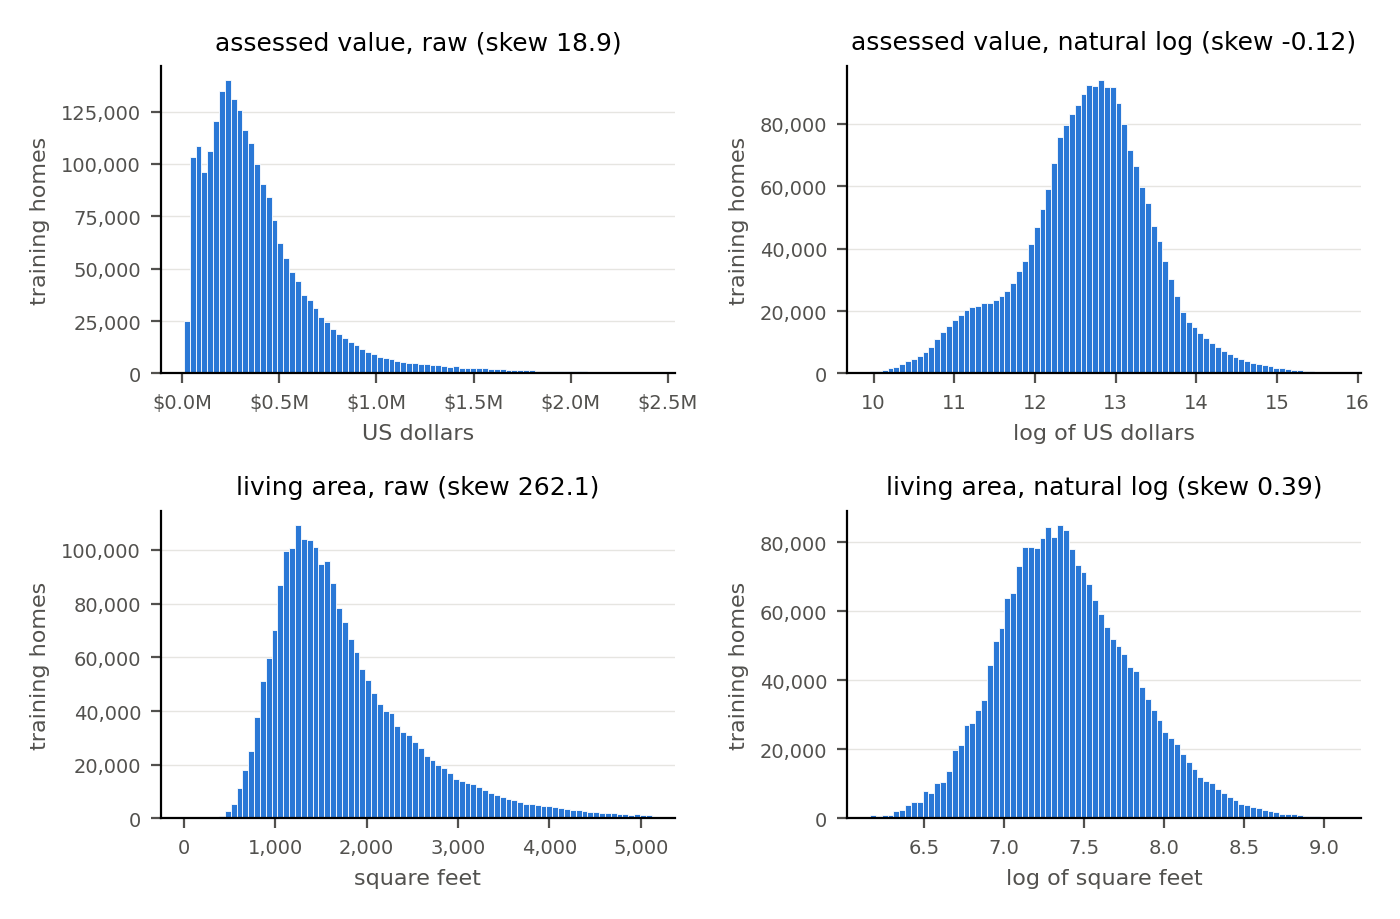
\includegraphics[width=0.82\textwidth]{figures/distributions.png}
\caption{The assessed value (top) and the living area (bottom) of the 2,287,442 training homes, raw and after the natural log. Raw panels stop at the 99th percentile (\$2.42 million and 5,120 square feet) so the bars stay visible; log panels drop the outer 0.1\% on each side. Each skew is computed on every training home.}
\label{fig:distributions}
\end{figure*}

\subsection{Which homes are kept}
Phase 2 kept every row that had a label, which let in shops, parcels with no building and assessed values of one dollar. We now keep only ordinary homes with a building on them. The rules in Table~\ref{tab:rows} run in order and each removed home is counted once, under the first rule it fails. The kept property types are single family, condominium, duplex, triplex, quadruplex, planned unit development, mobile home, cluster home, residential general, cooperative, manufactured home and townhouse.

\begin{table}[t]
\caption{Row rules, applied in order.}
\label{tab:rows}
\small
\begin{tabular}{@{}lr@{}}
\toprule
Rule & Homes removed \\
\midrule
No assessed value & 34,266 \\
Assessed in a year other than 2016 & 3,379 \\
Assessed value under \$10,000 & 14,505 \\
Not a residential home, or no type & 13,768 \\
No living area recorded (no building) & 25,926 \\
Zero bedrooms or no bathroom & 34,071 \\
\midrule
Homes kept & 2,859,302 \\
\bottomrule
\end{tabular}
\end{table}

\subsection{Training homes, test homes and folds}
The kept homes were shuffled with seed 42 and split 80/20: 2,287,442 training homes and 571,860 test homes. Each parcel appears exactly once in the file, so no home can sit on both sides of the split. The test homes were sealed. No setting, feature or rule was chosen by looking at them, and each final model was scored on them once.

The training homes were divided into five folds of about 457,000 homes each (457,575, 456,676, 457,411, 458,657 and 457,123), using a hash of the parcel number so that a home always lands in the same fold.

\subsection{Features}
The 17 features fall into three kinds.
\begin{itemize}
\item \textbf{Seven numbers}: bathrooms, bedrooms, year built, log living area, log lot area, stories and fireplaces. Each is standardized with the training average and spread.
\item \textbf{Two yes/no columns}: pool, and hot tub or spa.
\item \textbf{Eight categories}, one-hot encoded: ZIP code, zoning, neighbourhood, county land-use code, census tract, building quality, heating and air conditioning. A value held by fewer than 0.1\% of training homes joins an ``other'' value, a blank becomes its own value (``not recorded''), and the most common value of each group is dropped as the baseline.
\end{itemize}

Several columns are blank for a reason rather than at random. Los Angeles never records garage area, fireplaces or stories, while Orange and Ventura never record building quality or zoning. A blank fireplace count in Orange means no fireplace; in Los Angeles it means nobody counted. We handled each column by what its blanks mean (Appendix~\ref{app:fixes}, Fix 6), and the ZIP code and land-use columns tell the models which county a home is in.

The census tract comes from the raw tract-and-block number with the block digits removed. Every list of values and every fill-in value was learned from the training homes only.

\subsection{Correlation checks}
\label{sec:checks}
The association between two columns was measured by the Pearson correlation for two numbers, by the correlation ratio for a category and a number, and by the bias-corrected Cram\'er's V for two categories \cite{cramer1946,bergsma2013}. The correlation ratio of a many-valued category is inflated when it is measured on the homes it was fitted on, so it was measured on fold 0 after fitting the category averages on the other four folds. Figure~\ref{fig:heatmap} in the appendix shows every pair.

Four rules then decided which features stay.
\begin{enumerate}
\item No feature may reach 0.85 with the label (the professor's rule). None did; the strongest is the log living area at 0.525.
\item When two features reach 0.85 with each other, the one weaker with the label is dropped, strongest pair first. Six were dropped: county (0.998 with the county land-use code), miles east (0.988 with ZIP code), miles north (0.983 with ZIP code), property type (0.935 with the land-use code), city (0.921 with ZIP code) and garage area (0.906 with the land-use code).
\item A dropped column comes back if it lies between 0.60 and 0.80 with the label and stays under 0.85 with every kept feature. Only the three leak columns sat in that window, and they are barred (below), so nothing came back.
\item After one-hot encoding, the same pair rule ran on the model columns and removed 28 of them, mostly a neighbourhood or census tract that covers exactly the same homes as one ZIP code. The smallest eigenvalue of the column correlation matrix is 0.0041, so no column is an exact combination of the others.
\end{enumerate}

Three columns were removed by name before any rule ran: the building value, the land value and the tax amount. The first two add up to the label exactly and the tax bill is about 1\% of it. On the log label they measure only 0.583 to 0.653, under the 0.85 limit, because they are in dollars and the label is a log. The rule alone would have let them in.

%% ---------------------------------------------------------------------------------------------------------------
\section{Experimental Setup}
\label{sec:setup}

\subsection{One protocol for every model}
Every model went through the same four steps.
\begin{enumerate}
\item \textbf{Search.} Each setting in the model's grid trains on four folds and is scored on the fifth, five times, so every training home is used for validation exactly once \cite{kohavi1995}.
\item \textbf{Winner.} The setting with the lowest average validation mean squared error (MSE) of the log value wins, counting only settings scored on all five folds.
\item \textbf{Final fit.} The winning setting is trained once on all 2,287,442 training homes.
\item \textbf{Test.} The final model is scored once on the 571,860 test homes.
\end{enumerate}
The winner is picked on MSE of the log because most of the models minimise squared error during training, and on the log scale it measures relative misses. Linear regression has no setting to search, but it still ran on all five folds so its validation score is comparable. The two baselines were validated on fold 0 only.

\subsection{Scores}
For each model we report the MSE and the coefficient of determination ($R^2$) on the log value, $R^2$ and the root mean squared error (RMSE) in dollars, the median miss as a percentage of the true value, and the share of homes predicted within 20\% of their value. $R^2$ in dollars is pulled around by the most expensive homes, which is why the selection works on the log.

\subsection{Price bands for the classification models}
The brief asks a regression project to also try classifiers on a discretised label. We cut the log value into five bands of equal size at the training quintiles. The edges fall at \$165,080, \$269,041, \$387,279 and \$580,090, and each band holds about 457,400 training homes. Seven classifiers were trained on these bands with the same four steps, choosing the winner by the highest average validation accuracy. Logistic regression, the perceptron, naive Bayes and the Bayesian network used every training home. To fit the time available, K-nearest neighbours and the mixture of experts were trained on a random sample of 100,000 training homes and the linear support vector classifier on 20,000 (seed 42). All seven were tested on all 571,860 test homes. Each regression model's test predictions were also cut at the same edges, so every model appears in one band table. Band results report accuracy, the macro-averaged F1 score (equal weight to each band) and the share of homes placed within one band of the true band.

\subsection{Regression and classifier forms}
\label{sec:forms}
The slides teach linear regression as a regression model, and decision trees and random forests in both forms (Lecture 10). They teach K-nearest neighbours, the support vector machine and the ensembles of Lecture 13 as classifiers only. We first ran every model that has a regression form on the log value, because one score, the MSE of the log, can then rank them all. We then trained on the bands the classifier forms the slides teach for K-nearest neighbours and the support vector machine, and two models from the slides we had not run, the mixture of experts and the Bayesian network (Section~\ref{sec:slideforms}). The classifier forms of bagging, AdaBoost and voting, and the ID3 tree of Lecture 9, were not trained in this phase, so those three ensembles appear in regression form only.

\subsection{Hardware and software}
Everything ran on an Apple M1 Pro laptop with 16 GB of memory. The code is Python 3.12 with scikit-learn 1.8 \cite{pedregosa2011} and PyTorch 2.11 \cite{paszke2019}, which ran the neural network and the nearest-neighbour search on the laptop's graphics processor. Every random step uses seed 42 (or 42 plus the fold number), so a rerun repeats the same splits, samples and starting weights.

The memory limit shaped several grids. A fully grown regression tree on 1.8 million homes has two to three million nodes, so a forest of 50 such trees would not fit in 16 GB. The grids in Table~\ref{tab:grids} are therefore smaller than we would choose on a larger machine, and each limit is explained in the model's section.

\begin{table*}[t]
\caption{Every model, the lecture it comes from, the settings searched, what was held fixed, and the setting that won on validation.}
\label{tab:grids}
\small
\renewcommand{\arraystretch}{1.15}
\begin{tabularx}{\textwidth}{@{}L{2.6cm}L{0.9cm}YYL{3.1cm}@{}}
\toprule
Model & Lecture & Settings searched & Held fixed & Winner \\
\midrule
Average and median baselines & -- & none & predict one number for every home & -- \\
Linear regression & 4 & none & ordinary least squares, all 606 columns & -- \\
Neural network & 7 & hidden layers 256--128, 128--64, 512--256; dropout 0 or 0.2; SGD at learning rate 0.1 or Adam at 0.001 (12 settings) & ReLU; batch 1,024; MSE loss; at most 100 passes; stop after 5 passes without improvement & 256--128, Adam 0.001, dropout 0.2 \\
K-nearest neighbours & 3 & $k$ = 1, 3, 5, 10, 15, 20, 30, 50; Euclidean or cosine distance (16 settings) & exact search; prediction = mean log value of the $k$ neighbours & $k$ = 50, Euclidean \\
Decision tree & 9, 10 & smallest leaf 1, 5, 20, 50, 200 homes & squared-error splits; no depth limit & smallest leaf 200 \\
Random forest & 10, 13 & columns per split: square root (24), 10\% (60), 33\% (199) & 50 trees; bootstrap samples; smallest leaf 5 & 10\% (60 columns) \\
Bagging & 10, 13 & none & a forest that may split on all 606 columns; 50 trees; smallest leaf 5 & -- \\
Support vector machine & 12 & penalty $C$ = 0.01 or 1; margin width $\epsilon$ = 0 or 0.05 (4 settings) & linear kernel; $\epsilon$-insensitive loss; at most 2,000 passes & $C$ = 0.01, $\epsilon$ = 0.05 \\
AdaBoost.R2 & 13 & tree depth 4 or 8 & 50 rounds; linear loss & depth 8 \\
K-means clustering & 14 & 50, 200 or 1,000 clusters & mini-batches of 4,096; 3 restarts; home priced at its cluster's median & 1,000 clusters \\
Hierarchical clustering & 14 & 50, 200 or 1,000 clusters & Ward linkage on 10,000 sampled homes; home joins nearest cluster centre & 1,000 clusters \\
Voting & 13 & none & average of the three regression models with the best validation scores & neural network, random forest, K-nearest neighbours \\
Logistic regression & 5 & penalty $C$ = 0.01, 1, 100 & five bands; L2 penalty; at most 300 passes & $C$ = 1 \\
Perceptron & 6 & 5 or 20 passes & five bands, one against the rest; no penalty & 5 passes \\
Naive Bayes & 11 & smoothing 0.1, 1, 10 & five bands; normal model for numbers, yes/no model for 0/1 columns & smoothing 0.1 \\
K-nearest neighbours, vote & 3 & $k$ = 1 to 50; Euclidean or cosine & majority vote; MinMax scaling; 100,000-home sample & $k$ = 30, Euclidean \\
Linear SVM classifier & 12 & $C$ = 0.01, 0.1, 1, 10 & hinge loss; soft margin; one per band; 20,000-home sample & $C$ = 0.1 \\
Mixture of experts & 13 & 2, 4 or 8 experts & linear softmax experts; softmax gate; Adam 0.001; 100,000-home sample & 8 experts \\
Bayesian network & 11 & four parent sets for the band & counting with Laplace smoothing; all homes & ZIP code, living area, quality, year built \\
\bottomrule
\end{tabularx}
\end{table*}

%% ---------------------------------------------------------------------------------------------------------------
\section{The Models One by One}
\label{sec:models}

Each subsection gives the model's setup and why its settings were chosen, its validation and test results, and how well it fits this problem. Each one ends with a verdict: whether the result is good or bad, why, and what we would change next. We judge every model against three marks on the test homes: the median baseline (MSE of the log 0.702), linear regression (0.394) and the best model (0.373). Section~\ref{sec:top} explains why no model here gets far below 0.37. Table~\ref{tab:test} collects the test scores.

\subsection{Baselines}
The average baseline predicts the average training value in dollars for every home, and the median baseline predicts the median. They learn nothing about homes, so they mark the score a model must beat to have learned anything. On the test homes the median baseline misses by a median of 45.4\% (MSE of the log 0.702) and the average baseline by 53.8\% (0.828). The average baseline's $R^2$ on the log is negative ($-0.18$): the average dollar value sits above the typical home, because a few very expensive homes pull it up.

\emph{Verdict.} Both are bad by design. They set the floor, and every trained model beats them; even the weakest, AdaBoost at 0.4903, cuts the median baseline's error by 30\%.

\subsection{Linear regression}
Ordinary least squares fits one weight per model column \cite{hastie2009}. It has no setting to tune, so it ran on the five folds only to give a comparable validation score. The five fold scores sit between 0.3928 and 0.3952 (average 0.3943, spread 0.0010), and the test score is 0.3944, with $R^2 = 0.436$ on the log and a median miss of 33.8\%. Thirty percent of test homes land within 20\% of their value.

Linear regression cuts the median baseline's error by 44\% using nothing but additive effects. On the log scale each column adds a fixed percentage to the value, so a ZIP code adds the same percentage to a small condominium as to a large house. The model cannot learn that the price of an extra square foot depends on where the home is. That limit is its main weakness here. In its favour, it fits in seconds and every weight can be read and checked.

\emph{Verdict: good for so simple a model.} At 0.3944 it is only 0.0219 behind the best model, and it is the steadiest result in the study: a fold spread of 0.0010 and a test score within 0.0001 of validation. Two choices in our pipeline made a straight line work this well. The log label turns each column's effect into a percentage, and the one-hot location groups let every ZIP code, neighbourhood and tract carry a percentage of its own. What it cannot do is combine columns. Next we would add interaction columns, such as living area within each county, and a finer location signal through target encoding of the census block (Section~\ref{sec:limits}).

\subsection{Neural network}
The network is a fully connected feed-forward network trained by backpropagation \cite{rumelhart1986}: 606 inputs, two hidden layers with the ReLU activation, dropout after each hidden layer \cite{srivastava2014}, and one output for the log value. Training minimises the squared error in batches of 1,024 homes, reshuffled every pass. A run stops when the validation error has not improved for five passes, at most 100, and keeps the weights from its best pass.

The grid crosses three sizes with two dropout rates and two optimisers. Plain stochastic gradient descent (SGD) ran at a learning rate of 0.1, and Adam \cite{kingma2015} at 0.001, the rate its authors recommend. Twelve settings on five folds made 60 runs, which took 3.5 hours on the laptop's graphics processor. Table~\ref{tab:nn} shows every setting.

\begin{table}[t]
\caption{Neural network search: average over the five validation folds, best first. Spread is the standard deviation of the five fold scores.}
\label{tab:nn}
\small
\setlength{\tabcolsep}{3pt}
\begin{tabular}{@{}lrrrrr@{}}
\toprule
Setting & MSE & Spread & $R^2$ & Median & Best \\
 & (log) & & (log) & miss \% & pass \\
\midrule
256--128 Adam, drop 0.2 & 0.3730 & 0.0010 & 0.467 & 32.4 & 27 \\
128--64 Adam, drop 0.2 & 0.3731 & 0.0011 & 0.467 & 32.4 & 38 \\
512--256 Adam, drop 0.2 & 0.3737 & 0.0014 & 0.466 & 32.5 & 27 \\
512--256 SGD, drop 0.2 & 0.3759 & 0.0033 & 0.463 & 32.8 & 39 \\
256--128 SGD, drop 0 & 0.3760 & 0.0029 & 0.463 & 32.9 & 14 \\
256--128 SGD, drop 0.2 & 0.3760 & 0.0026 & 0.463 & 32.7 & 28 \\
512--256 SGD, drop 0 & 0.3765 & 0.0025 & 0.462 & 33.0 & 18 \\
128--64 SGD, drop 0 & 0.3766 & 0.0028 & 0.462 & 33.0 & 29 \\
128--64 SGD, drop 0.2 & 0.3770 & 0.0019 & 0.461 & 32.7 & 31 \\
128--64 Adam, drop 0 & 0.3788 & 0.0020 & 0.459 & 33.0 & 19 \\
256--128 Adam, drop 0 & 0.3790 & 0.0008 & 0.459 & 32.7 & 21 \\
512--256 Adam, drop 0 & 0.3798 & 0.0006 & 0.457 & 33.0 & 20 \\
\bottomrule
\end{tabular}
\end{table}

Dropout decided the ranking more than size did. With Adam, adding dropout moved every size from last place to first, most likely because Adam without it fits the training folds quickly and then starts to memorise them. Those runs reached their best around pass 20 and did not improve after it. With SGD at 0.1 the noisy updates already act as a brake, and dropout changed little. The top three settings differ by 0.0007, less than the spread between folds, so they are effectively tied, and we took the listed winner without reading more into the order.

The final network (256--128, Adam, dropout 0.2) trained from fresh weights on all training homes for 27 passes, the median best pass of its five runs, in 4.5 minutes. On the test homes it scored an MSE of 0.3725 on the log ($R^2 = 0.467$), a median miss of 32.5\%, 31.6\% of homes within 20\%, and $R^2 = 0.569$ in dollars with an RMSE of \$405,643. That is 5.6\% lower error than linear regression on the log scale.

The network can combine location with size and age, which linear regression cannot, and it trains on all 2.3 million homes in minutes because it reads them in batches. It is harder to explain to a homeowner than a list of weights, it depends on the optimiser and learning rate being right, and runs on the graphics processor can differ in the last digits between reruns.

\emph{Verdict: good, the best model in the study.} It has the lowest validation and test error (0.3730 and 0.3725) and the best $R^2$ in dollars (0.569). Three parts of the process got it there. The search showed that dropout mattered most: with Adam, every size without dropout ranked last (0.3788 to 0.3798) and every size with it ranked first. Early stopping on the validation fold kept each run from training past its best pass. Training in batches let it learn from all 2.3 million homes. More tuning is unlikely to move it much, because the three best sizes are tied within 0.0007, and its remaining error looks like the label's rather than the model's (Section~\ref{sec:top}). The gains we would look for are in the data: a finer location signal, for example a learned embedding of the census block, and a label closer to market value if one can be found.

\subsection{K-nearest neighbours}
A home is priced at the mean log value of the $k$ training homes closest to it in the 606-column space \cite{cover1967}. Training only stores the homes, so all eight values of $k$ were scored from one neighbour search per distance. The search is exact, computed on the graphics processor in batches of 204 query homes against the 1.8 million homes of each fitting fold. Cosine distance compares the direction of two homes' columns and ignores their length, which is a different idea of ``similar'' from Euclidean distance; both were tried.

The best setting was $k = 50$ with Euclidean distance, at a validation MSE of 0.3853, and the final model scored 0.3839 on the test homes (median miss 33.2\%). Small $k$ copied the label noise. With a single neighbour the validation MSE was 0.7307, worse than predicting the median for every home, and the error fell at every step up to $k = 50$, the largest value in the grid. It was still falling there (0.3872 at $k = 30$), so a larger $k$ might have done slightly better. The two distances were tied at every $k$ (0.3859 for cosine against 0.3853 at $k = 50$), most likely because 597 of the 606 columns are one-hot, so under either measure the distance mostly counts the groups two homes do not share. The model is easy to explain, since each prediction can be traced to real neighbouring homes. It is slow to query, though, because each new home is compared with every training home, and every one-hot column counts as much as the living area in the distance.

\emph{Verdict: good, third on validation.} At 0.3839 it beats linear regression with no training at all. The choice of $k$ made it work: averaging 50 neighbours smooths away the noise a single neighbour copies (0.7307 at $k = 1$). One-hot location helped too, since the nearest homes usually share a ZIP code. Its weaknesses are cost and weighting. The final run took 45 minutes, almost all of it spent searching neighbours, and every column counts the same in the distance. Next we would extend the grid past $k = 50$, where the error was still falling, weight each neighbour by its distance, and scale the column groups so that location and size count by how much they matter.

\subsection{Decision tree}
A regression tree splits the homes in two again and again, choosing each split to cut the squared error most, and predicts the average log value of the homes in a leaf \cite{breiman1984}. We controlled its size by the smallest number of homes a leaf may hold. Pruning a grown tree by cost complexity would have been closer to the lecture, but a single full tree here takes about three minutes and the pruning grid would have taken days.

Leaf size mattered a great deal. With one home per leaf the tree memorised the training folds and scored 0.724 on validation, nearly twice the error of linear regression. A minimum of 5 homes gave 0.531, a minimum of 20 gave 0.433, and minimums of 50 and 200 gave 0.4137 and 0.4136, tied within the fold spread of about 0.0015. The final tree (smallest leaf 200), fitted on all training homes in 15.6 minutes, scored 0.4109 on the test homes ($R^2 = 0.412$ on the log) with a median miss of 34.7\%.

A tree reads like a set of rules a valuer would recognise, and it needs no scaling. Here, though, a single tree is beaten by linear regression, because it gives every home in a leaf the same value and so predicts in steps. Its main role in this study is as the building block of the forest, bagging and AdaBoost.

\emph{Verdict: weak on its own.} At 0.4109 it trails linear regression. A tree predicts in steps, one value per leaf, and the leaves had to hold 200 homes before it stopped memorising noise. The search over leaf size is what made it usable at all, since one home per leaf scored 0.724. Cost-complexity pruning on a sample of homes is the next thing to try, but the larger gain comes from averaging many trees, as the next sections show.

\subsection{Random forest}
A random forest averages many trees, each grown on a bootstrap sample of the homes and allowed to split on only a random share of the columns at each split \cite{breiman2001}. We searched that share (24, 60 or 199 of the 606 columns) and fixed 50 trees with at least 5 homes per leaf. One forest tree grown to single-home leaves on these homes has about two million nodes; with 5 homes per leaf it has about 276,000, which is what lets 50 of them fit in memory.

The best share was 10\% of the columns, 60 per split (validation MSE 0.3799), and the final forest scored 0.3788 on the test homes with a median miss of 32.6\%. Averaging fixed most of the single tree's overfitting. A single tree with 5-home leaves scored 0.531 on validation, yet 50 such trees averaged together scored 0.3799, ahead of the best single tree (0.4136) and of linear regression (0.3943). The middle share won: 24 columns scored 0.3831 and 199 scored 0.3861. With too few columns each tree is weak, and with too many the trees grow alike, so their errors stop cancelling when they are averaged. Forests are strong on tabular data and rarely need careful tuning. They are large in memory, slow to train on this many homes, and much harder to read than one tree.

\emph{Verdict: good, second on validation.} At 0.3788 the forest is the best tree model by a wide margin, 0.0321 ahead of the single tree. Two choices made it work: averaging 50 trees removes most of each tree's noise, and the search over the column share found the setting, 60 columns per split, where each tree is strong but the trees still differ. Memory was the limit. With 16 GB we could not grow deeper trees or more of them, and the final forest took 21 minutes. On a larger machine we would try more trees with smaller leaves, and compare against gradient-boosted trees, which the course does not cover.

\subsection{Bagging}
Bagging is the same forest with every column available at every split \cite{breiman1996}, so the trees differ only through their bootstrap samples. Comparing it with the random forest shows how much the random column choice adds. Bagging scored 0.3962 on validation and 0.3953 on the test homes, behind the forest (0.3799) and even slightly behind linear regression. With every column open at every split, the trees most likely choose the same strong columns, living area and ZIP code, near the top, so they make similar mistakes and averaging cancels fewer of them. It was also the slowest final fit of any model: 1.9 hours, against 21 minutes for the forest.

\emph{Verdict: bad next to the forest.} It trails the forest by 0.0165 and took five times as long. The cause is the one this comparison was built to show: without a random choice of columns the trees are too much alike. As a control, bagging did its job. The fix is the forest itself; if bagging had to stay, smaller bootstrap samples would at least cut its time.

\subsection{Support vector machine}
A linear support vector machine for regression ignores misses smaller than a margin $\epsilon$ and penalises larger ones in proportion to their size, weighted by $C$ \cite{cortes1995}. A kernel version would need a comparison between every pair of the 1.8 million homes, so we used the linear solver built for large data \cite{ho2012}. We searched $C$ (0.01 or 1) and $\epsilon$ (0 or 0.05 on the log scale, where 0.05 means misses under about 5\% cost nothing). The best setting was $C = 0.01$ with $\epsilon = 0.05$, at a validation MSE of 0.4120, and the test score was also 0.4120. All four settings scored between 0.4120 and 0.4125, inside one fold spread, so neither the penalty nor the margin mattered. The model did not land close to linear regression; it finished 0.018 behind it. Its loss grows with the size of a miss rather than with its square, so it fits the median home rather than the mean. The scores show this: it has the best median miss of any model (31.6\%) but a worse squared error, which is the score we rank on.

\emph{Verdict: mixed.} Ranked by squared error it is sixth on validation (0.4120), but it has the best median miss of every model (31.6\%) and the largest share of homes within 20\% (32.2\%). Both come from its loss: a miss counts by its size, not its square, so the few homes with huge misses, many of them probably mislabelled, do not pull the fit around. On this label that is a strength. The weakness is the linear kernel, which cannot combine columns. Next we would approximate a nonlinear kernel with random features, which keeps the cost manageable on this many homes, and report the median miss beside the MSE when ranking models.

\subsection{AdaBoost}
AdaBoost.R2 \cite{freund1997,drucker1997} fits trees one after another, drawing each round's sample so that the homes earlier rounds missed most appear more often, and combines the rounds by a weighted median. We ran 50 rounds and searched the depth of each tree (4 or 8). The best depth was 8 (validation MSE 0.4843; depth 4 scored 0.5017), and the test score was 0.4903, the weakest of the supervised models and behind a single tree. Its fold spread was also the largest we measured: 0.0048 at depth 8 and 0.0085 at depth 4. Each round gives more weight to the homes earlier rounds missed. In this file many of those are probably homes whose assessed value lags their market value, so boosting spends its rounds on errors no feature can explain.

\emph{Verdict: bad, the weakest supervised model.} At 0.4903 it is behind even a single tree, and its fold spread is the largest in the study, so it is also the least predictable. Boosting assumes that the homes it misses are hard but learnable. Here many of them are probably homes whose label no feature can explain, and AdaBoost.R2 samples them more and more often. We would replace it with gradient boosting under a loss that caps the pull of large misses, such as the Huber loss, and a small learning rate, so that no single home can dominate the later rounds.

\subsection{K-means clustering}
Clustering is unsupervised, so we turned it into a predictor: the training homes are grouped into $k$ clusters without looking at the label, and a home is priced at the median log value of the training homes in its cluster. K-means \cite{lloyd1982} ran in mini-batches of 4,096 homes \cite{sculley2010}, which keeps it fast on 1.8 million rows, with three restarts. The best number of clusters was 1,000 (validation MSE 0.4541), and the test score was 0.4532. More clusters helped at every step (0.5074 with 50, 0.4778 with 200), and 1,000 was the largest value tried. Even so, the model trails linear regression by 0.059 on the test homes. The clusters are formed without looking at the label, and every home in a cluster gets the same price.

\emph{Verdict: bad, as expected for a model that never sees the label.} The clusters group homes that look alike across 606 columns, not homes that cost alike, and every home in a cluster gets one price. Since more clusters helped at every step, the next run should go past 1,000. The better use of the clusters is probably as an extra column for a supervised model rather than as the predictor itself.

\subsection{Hierarchical clustering}
Ward's agglomerative method \cite{ward1963} merges the two clusters whose merge adds the least spread, starting from single homes. It needs the distance between every pair of homes, about $1.7 \times 10^{12}$ pairs for all the training homes, so we built the hierarchy on a random sample of 10,000 and then assigned every home to the nearest cluster centre. Prices come from cluster medians, as in K-means. The best number of clusters was 1,000 (validation MSE 0.4559), and the test score was 0.4556. At every number of clusters it finished within 0.002 of K-means, so building the hierarchy on a sample cost little overall. The sample is still the obvious weakness: a cluster structure learned from about half a percent of the homes may miss small expensive neighbourhoods.

\emph{Verdict: bad, for the same reason as K-means.} Its 0.4556 is within 0.003 of K-means, so the 10,000-home sample cost little, but one price per cluster still holds it back. With more memory we would build the hierarchy on a larger sample. The bigger change is the one proposed for K-means: use the clusters as a feature, not as the prediction.

\subsection{Voting}
Voting averages the log predictions of the three regression models with the lowest average validation MSE \cite{dietterich2000}. The members were picked on validation scores only, so the test homes still played no part. The members were the neural network, the random forest and K-nearest neighbours, and the vote scored 0.3731 on the test homes. Voting has no validation score of its own, so it cannot be ranked against the other models on validation and is reported on the test homes only. It did slightly worse than the network alone (0.3725). Averaging helps when the members make different mistakes, and these three do not: the correlation between any two members' test errors is 0.977 to 0.981, and 88\% of the network's worst tenth of homes are also among the forest's worst tenth. So the vote pulled the network toward its two weaker partners rather than cancelling errors.

\emph{Verdict: no gain.} It is second on the test homes but 0.0006 worse than the network alone. Our rule chose members by validation score only, which picks three good models but not three different ones. Next time we would pick members whose errors differ, for example a model with a different loss such as the support vector machine, or learn the weight of each member on the validation folds instead of averaging equally.

\subsection{Logistic regression}
\label{sec:logistic}
Logistic regression \cite{cox1958} is the first of the three classifiers. It predicts a price band, not a value. For each of the five bands it computes a linear score from the 606 columns, turns the five scores into probabilities with the softmax function, and gives the home the most probable band. Training minimises the cross-entropy between those probabilities and the true bands, with an L2 penalty on the weights whose strength is set by $C$; a smaller $C$ means a stronger penalty. We searched $C$ = 0.01, 1 and 100 with the L-BFGS solver and at most 300 passes. Guessing the most common band would be right about 20\% of the time.

\begin{table}[t]
\caption{Logistic regression search: average over the five validation folds. Spread is the standard deviation of the five accuracies.}
\label{tab:logistic}
\small
\setlength{\tabcolsep}{4pt}
\begin{tabular}{@{}lrrrrr@{}}
\toprule
$C$ & Accuracy & Spread & Macro & Within one & Seconds \\
 & (\%) & & F1 & band (\%) & per fold \\
\midrule
0.01 & 41.04 & 0.04 & 0.396 & 75.08 & 67 \\
1 & 41.16 & 0.05 & 0.397 & 75.26 & 129 \\
100 & 41.16 & 0.04 & 0.397 & 75.27 & 126 \\
\bottomrule
\end{tabular}
\end{table}

$C = 1$ won with an average validation accuracy of 41.16\% (Table~\ref{tab:logistic}), ahead of $C = 100$ by less than 0.01 points and of $C = 0.01$ by 0.12. The penalty hardly mattered: with 2.3 million training homes and 606 columns the model has little room to overfit, so a penalty has little to correct. One caveat. With $C$ = 1 and 100, every fit, the final one included, stopped at the 300-pass limit before the solver's convergence test was met; with $C$ = 0.01 it converged. Because the three settings score almost the same, more passes would probably change little, but we did not test it.

The final model was fitted and scored in 2.8 minutes. It placed 41.2\% of test homes in the right band, with a macro F1 of 0.398, and 75.3\% within one band. That beats every regression model cut into bands, the best of which is the neural network at 38.8\%; of the models trained on the bands, only the Bayesian network and the mixture of experts did better (Section~\ref{sec:slideforms}). Logistic regression is trained for exactly this task, while the regression models are trained to get the value close, not to land on the right side of a band edge. On the looser score the regression models win: the network puts 81.8\% of homes within one band.

\begin{table}[t]
\caption{Logistic regression on the test homes: the share of each true band given each predicted band. Rows add up to 100\%.}
\label{tab:logistic-bands}
\small
\setlength{\tabcolsep}{4pt}
\begin{tabular}{@{}lrrrrr@{}}
\toprule
True band & 1 & 2 & 3 & 4 & 5 \\
\midrule
1 (under \$165,080) & \textbf{46.6} & 22.2 & 7.5 & 14.3 & 9.4 \\
2 & 32.9 & \textbf{32.5} & 14.0 & 13.9 & 6.7 \\
3 & 24.5 & 21.3 & \textbf{17.8} & 25.8 & 10.7 \\
4 & 18.4 & 8.1 & 13.8 & \textbf{35.9} & 23.7 \\
5 (over \$580,090) & 7.3 & 0.9 & 1.6 & 16.7 & \textbf{73.4} \\
\bottomrule
\end{tabular}
\end{table}

Table~\ref{tab:logistic-bands} shows where it goes wrong. The dearest band is the easiest (73.4\% correct) and the middle band the hardest (17.8\%), because a middle band can be confused with a neighbour on either side. The cheapest band shows the label problem again: 23.7\% of its homes are placed in band 4 or 5, at least three bands too high. A home bought decades ago in an expensive area keeps a low assessed value under Proposition 13 while its features describe an expensive home. That is the likely cause, though the file cannot confirm it.

\emph{Verdict: good at its own task, with two weaknesses.} It beats every regression model at the exact band (41.2\%), because it is trained to choose a band; only the Bayesian network and the mixture of experts, also trained on the bands, do better. First, it treats the five bands as unordered labels, so placing a band-1 home in band 5 costs no more than placing it in band 2. That is likely one reason 9.4\% of band-1 homes land in band 5. An ordinal model, which knows the bands are ordered, would be our next step. Second, the two weaker penalties stopped at the pass limit; a rerun with more passes would confirm that the score has settled.

\subsection{Perceptron and naive Bayes}
The perceptron \cite{rosenblatt1958} learns one linear boundary per band against the rest, and we searched 5 or 20 passes. Naive Bayes \cite{domingos1997} treats the columns as independent within a band. It uses a normal distribution for each of the seven standardized numbers and a yes/no probability for each 0/1 column, with smoothing 0.1, 1 or 10.

The perceptron won with 5 passes (validation accuracy 33.90\%) and naive Bayes with smoothing 0.1 (38.39\%; the three smoothing values were within 0.03 points). On the test homes they placed 34.9\% and 38.5\% of homes in the right band, with macro F1 scores of 0.339 and 0.362 and 71.7\% and 70.6\% within one band. Both trail logistic regression. The perceptron was the least steady model in the study. Its validation accuracy varied by 1.8 points between folds with 5 passes and by 3.1 with 20, against 0.05 or less for the other two classifiers. When straight boundaries cannot separate the bands, the perceptron never settles, so where it stops depends on the last homes it saw; 20 passes did worse (31.72\%). Naive Bayes trails logistic regression by 2.8 points. Its independence assumption is badly broken here: ZIP code, neighbourhood, census tract and zoning all describe the same place, and the model counts that evidence several times.

\emph{Verdict: both bad, for different reasons.} The perceptron (34.9\%) is the weakest classifier and the least steady, because it has no probability to optimise and never settles on bands that straight lines cannot separate. The usual fix is the averaged perceptron, which averages its weights over every pass. Naive Bayes (38.5\%) is the fastest classifier, 6 seconds for the final fit, but its independence assumption double-counts location. Giving it a single location group, ZIP code, would be the first thing to try.

\subsection{K-nearest neighbours as a classifier}
\label{sec:slideforms}
The next four models were trained on the bands in the form the slides teach. This one is Lecture 3's: a home gets the most common band among its $k$ nearest training homes, and the features are MinMax scaled, so each of the seven number columns runs from 0 to 1 over the homes the model is fitted on. A tie goes to the tied band that holds the nearest neighbour. We searched $k$ from 1 to 50 with Euclidean and cosine distance on a random sample of 100,000 training homes, and tested on all test homes.

$k = 30$ with Euclidean distance won (validation accuracy 39.27\%), and the final model placed 39.6\% of test homes in the right band (macro F1 0.386, 73.2\% within one band). A single neighbour scored 36.5\%. Accuracy rose steeply up to $k = 15$ and then levelled off between 39.1\% and 39.3\%. Euclidean matched or beat cosine at every $k$, by up to 0.6 points.

\emph{Verdict: fair, held back by its sample.} It beats naive Bayes and the perceptron but trails logistic regression by 1.7 points, and logistic regression saw 23 times as many homes. Trained for the band directly, the vote does better than its own regression form cut into bands (38.3\%), even with a twentieth of the homes. Next we would run it on every training home, about six hours of neighbour search on the laptop's graphics processor, and weight each column group by its importance in the distance.

\subsection{Linear support vector classifier}
This is the classifier Lecture 12 teaches: a maximum-margin hyperplane with the hinge loss. The bands overlap, so the hard margin of the slides has no solution; we used the soft margin, where each mistake costs $C$ times its distance past the margin. The slides cover two classes, so there is one machine per band against the rest. We searched $C$ = 0.01, 0.1, 1 and 10 on a random sample of 20,000 training homes and tested on all test homes.

$C = 0.1$ won (34.38\% on validation), and the test accuracy was 34.2\% (macro F1 0.294, 64.4\% within one band).

\emph{Verdict: bad, the weakest band model.} It trails logistic regression, also a linear model, by 7.1 points. It saw 20,000 homes, under a hundredth of what logistic regression saw, and its folds varied by 0.7 to 1.4 points, so the sample was too small to be steady. With $C$ of 0.1 and above, 11 of the 15 search fits stopped at 10,000 passes before converging; the final fit converged. The hinge loss also gives no probabilities, so the five machines are compared on raw scores that share no common scale. Next we would train it on every home, which the linear form allows in one to three hours, before judging the method itself.

\subsection{Mixture of experts}
Lecture 13 presents the mixture of experts as the answer to boosting's sequential training: several expert classifiers are trained at the same time on the same homes, and a gating network with a softmax decides how much to trust each expert for each home. Our experts are linear softmax classifiers over the 606 columns, and a band's probability is the gate-weighted sum of the experts' probabilities. Experts and gate were trained together with Adam at a learning rate of 0.001 in batches of 1,024, stopping when the error on 10\% of the fitting homes, held out for the purpose, had not improved for five passes. We searched 2, 4 or 8 experts on a random sample of 100,000 training homes and tested on all test homes.

Eight experts won (42.06\% on validation), and the final model placed 42.3\% of test homes in the right band (macro F1 0.411, 76.3\% within one band), second of all models.

\emph{Verdict: good.} With a twentieth of the homes it beats logistic regression trained on all of them (41.2\%). The gain comes from the gate: a mixture with a single expert is logistic regression, and accuracy rose with every expert added (41.31\%, 41.58\%, 42.06\%). A likely reason is that the three counties record different columns and price the same features differently, so experts that specialise in one part of the market help, and the gate lets them. Eight was the largest number tried and accuracy was still rising, so the next run should try more experts on every training home.

\subsection{Bayesian network}
Lecture 11 builds the network from causal relationships and learns each node's table by counting. A home's location, size, quality and age cause its value, so the price band is a child of those features. The slides say to try several structures and keep the best performing one, so we compared four parent sets for the band by five-fold cross-validation, each with ZIP code and living area, adding building quality, year built, or both. Number features were cut at the quintiles of the fitting homes. Each table entry is $P(\text{band} \mid \text{parents}) = (n + 1)/(N + 5)$, where $n$ counts the homes with that band and those parent values and $N$ the homes with those parent values; the $+1$ (Laplace smoothing) keeps an unseen band from probability 0. Every feature is known when a home is priced, so the prediction reads only the band's own table, and edges between features do not change it. One step goes beyond the slides: a home whose parent values never occur among the fitting homes falls back to fewer parents (back-off). The network only counts, so it ran on every training home in about 12 seconds per fold.

The four-parent structure won (42.44\% on validation): ZIP code, living area, building quality and year built. The final network placed 42.6\% of test homes in the right band (macro F1 0.411, 74.9\% within one band), the best exact-band score of any model.

\emph{Verdict: good, the best band model.} It leads the mixture of experts (42.3\%) and logistic regression (41.2\%), with a fold spread of only 0.10 points. The causal structure is what made it work: with only four parents each table entry is learned from many homes, and the table lets location and size combine, which a linear model cannot do. Each added parent helped: 40.74\% with two, 41.73\% or 42.09\% with three, 42.44\% with four. Year built helped more than building quality, possibly because older homes were more often bought long ago, which ties to the Proposition 13 effect. Its weakness is the size of its tables: every added parent multiplies the number of combinations, so a fifth parent would leave many combinations with too few homes. Next we would try more structures with the slide's ordering method, and finer location such as the census tract as a parent.

%% ---------------------------------------------------------------------------------------------------------------
\section{All Models Side by Side}
\label{sec:all}

\begin{table*}[t]
\caption{Every regression model on the 571,860 test homes, ranked by average validation MSE of the log (the baselines on fold 0 only). Each model was scored on the test homes once.}
\label{tab:test}
\small
\begin{tabular}{@{}lrrrrrrr@{}}
\toprule
Model & Validation MSE & Test MSE & Test $R^2$ & Test $R^2$ & RMSE & Median & Within \\
 & (log) & (log) & (log) & (\$) & (\$) & miss (\%) & 20\% (\%) \\
\midrule
Neural network & 0.3730 & 0.3725 & 0.467 & 0.569 & 405,643 & 32.5 & 31.6 \\
Random forest & 0.3799 & 0.3788 & 0.458 & 0.495 & 439,367 & 32.6 & 31.7 \\
K-nearest neighbours & 0.3853 & 0.3839 & 0.451 & 0.508 & 433,416 & 33.2 & 30.9 \\
Linear regression & 0.3943 & 0.3944 & 0.436 & 0.490 & 441,385 & 33.8 & 30.0 \\
Bagging & 0.3962 & 0.3953 & 0.435 & 0.543 & 417,993 & 33.2 & 31.5 \\
Support vector machine & 0.4120 & 0.4120 & 0.411 & 0.496 & 439,039 & 31.6 & 32.2 \\
Decision tree & 0.4136 & 0.4109 & 0.412 & 0.454 & 456,740 & 34.7 & 29.6 \\
K-means clustering & 0.4541 & 0.4532 & 0.352 & 0.354 & 496,685 & 34.6 & 29.8 \\
Hierarchical clustering & 0.4559 & 0.4556 & 0.349 & 0.350 & 498,451 & 34.7 & 29.8 \\
AdaBoost.R2 & 0.4843 & 0.4903 & 0.299 & 0.387 & 483,984 & 42.4 & 22.3 \\
Voting (top three) & -- & 0.3731 & 0.466 & 0.527 & 425,368 & 32.5 & 31.8 \\
Median baseline & 0.7011 & 0.7021 & $-0.004$ & $-0.036$ & 629,192 & 45.4 & 22.3 \\
Average baseline & 0.8261 & 0.8278 & $-0.184$ & 0.000 & 618,192 & 53.8 & 20.9 \\
\bottomrule
\end{tabular}
\end{table*}

\begin{table}[t]
\caption{Every model on the five price bands of the test homes. Band models were trained on the bands; regression models had their predictions cut at the same edges. $^{a}$Trained on 100,000 sampled homes; $^{b}$on 20,000.}
\label{tab:bands}
\small
\setlength{\tabcolsep}{4pt}
\begin{tabular}{@{}lrrr@{}}
\toprule
Model & Accuracy & Macro & Within one \\
 & (\%) & F1 & band (\%) \\
\midrule
\multicolumn{4}{@{}l}{\emph{Trained on the bands}} \\
Bayesian network & 42.6 & 0.411 & 74.9 \\
Mixture of experts$^{a}$ & 42.3 & 0.411 & 76.3 \\
Logistic regression & 41.2 & 0.398 & 75.3 \\
K-nearest neighbours, vote$^{a}$ & 39.6 & 0.386 & 73.2 \\
Naive Bayes & 38.5 & 0.362 & 70.6 \\
Perceptron & 34.9 & 0.339 & 71.7 \\
Linear SVM classifier$^{b}$ & 34.2 & 0.294 & 64.4 \\
\multicolumn{4}{@{}l}{\emph{Regression models, cut into bands}} \\
Neural network & 38.8 & 0.394 & 81.8 \\
Random forest & 38.7 & 0.393 & 81.6 \\
K-nearest neighbours & 38.3 & 0.390 & 81.1 \\
Linear regression & 37.3 & 0.379 & 80.7 \\
Bagging & 38.7 & 0.395 & 80.6 \\
Support vector machine & 38.7 & 0.383 & 82.4 \\
Decision tree & 36.7 & 0.371 & 80.0 \\
K-means clustering & 34.8 & 0.335 & 79.7 \\
Hierarchical clustering & 34.7 & 0.333 & 79.8 \\
AdaBoost.R2 & 30.6 & 0.300 & 70.8 \\
Voting (top three) & 38.8 & 0.394 & 81.8 \\
Median baseline & 20.0 & 0.067 & 60.0 \\
Average baseline & 20.1 & 0.067 & 60.1 \\
\bottomrule
\end{tabular}
\end{table}

Table~\ref{tab:test} ranks the regression models by validation and shows their test scores next to it. Table~\ref{tab:bands} shows the same comparison as a five-class problem. The neural network won, followed by the two models that average many predictions, the forest and K-nearest neighbours. The field is close, though. The network beats linear regression by only 0.0219 on the log scale, 5.6\% of linear regression's error, and apart from AdaBoost and the two clusterings every model lands between 0.3725 and 0.4120 on the test homes. The band table keeps roughly the same order among the regression models, but the top six sit within 0.6 points of each other, so the bands cannot separate them. The models trained on the bands themselves stand clear at the exact band: the Bayesian network (42.6\%), the mixture of experts (42.3\%) and logistic regression (41.2\%) all beat every regression model cut into bands.

%% ---------------------------------------------------------------------------------------------------------------
\section{The Top Three Models}
\label{sec:top}

Ranked by average validation MSE of the log, the three strongest models are the neural network, the random forest and K-nearest neighbours (Table~\ref{tab:top}). The network leads the forest by 0.0069 on validation, several times the fold spread of about 0.001, and the order holds on the test homes. For the forest and K-nearest neighbours the final time includes predicting the test homes; for K-nearest neighbours that prediction is nearly all of it, because training only stores the homes.

\begin{table}[t]
\caption{The three strongest models. Spread is the standard deviation of the five validation folds; county and band rows give the test median miss.}
\label{tab:top}
\small
\setlength{\tabcolsep}{4pt}
\begin{tabular}{@{}lrrr@{}}
\toprule
 & Neural & Random & K-nearest \\
 & network & forest & neighbours \\
\midrule
Validation MSE (log) & 0.3730 & 0.3799 & 0.3853 \\
Fold spread & 0.0010 & 0.0011 & 0.0013 \\
Test MSE (log) & 0.3725 & 0.3788 & 0.3839 \\
Test median miss (\%) & 32.5 & 32.6 & 33.2 \\
\quad Los Angeles & 33.6 & 33.9 & 34.5 \\
\quad Orange & 31.0 & 31.0 & 31.4 \\
\quad Ventura & 28.4 & 28.0 & 28.6 \\
\quad cheapest band & 162.6 & 162.0 & 155.5 \\
\quad dearest band & 35.8 & 36.4 & 36.8 \\
Final run (minutes) & 4.5 & 21.4 & 45.2 \\
\bottomrule
\end{tabular}
\end{table}

\subsection{Where the variability comes from}
\textbf{Between folds.} The five fold scores of one setting vary very little: the spread is 0.0010 for linear regression, between 0.0006 and 0.0033 for the network settings, and between 0.0011 and 0.0021 for the decision trees. Each fold holds about 457,000 homes, so a fold's average error is already a very stable number. The practical rule we draw from this is that two settings closer than about 0.002 are tied. The three best network settings fall inside that margin, and so do the decision trees with leaves of 50 and 200 homes. SGD runs varied more than Adam runs (0.0019 to 0.0033 against 0.0006 to 0.0014), and their best pass ranged from 14 to 39. A large fixed learning rate makes the error bounce from pass to pass, so where a run stops depends on luck.

\textbf{Between validation and test.} The test scores agree with validation to within a fold spread: 0.3730 against 0.3725 for the network, 0.3943 against 0.3944 for linear regression, 0.3799 against 0.3788 for the forest and 0.3853 against 0.3839 for K-nearest neighbours. AdaBoost moved the most, 0.0060 worse on the test homes, in line with its unusually large fold spread (0.0048). The test homes were never used to choose anything, so this agreement suggests the search did not overfit the folds. The decision tree did slightly better on the test homes than on validation (0.4109 against 0.4136). Its final fit saw all 2.3 million training homes instead of the 1.8 million of a fold, and with a fixed minimum of 200 homes per leaf, more homes allow more and finer leaves.

\textbf{Between models.} The differences between models are larger than the differences between folds, and they follow how each model handles noise. The decision tree with one home per leaf copies each training home's label, including its noise, and its error nearly doubles. Averaging (forest, bagging, voting) and larger leaves smooth that noise away. K-nearest neighbours shows the same pattern: one neighbour scored 0.7307 on validation and 50 neighbours 0.3853. The forest averages 50 trees with 5-home leaves, a leaf size that scored 0.531 as a single tree, and becomes the second-best model at 0.3799.

\textbf{Between parts of the market.} All three top models miss most in Los Angeles (median miss 33.6\% to 34.5\%) and least in Ventura (28.0\% to 28.6\%), with Orange in between (Table~\ref{tab:top}). One likely reason is that Los Angeles never records garage area, fireplaces or stories, so its homes are described by fewer columns; it also holds 68\% of the test homes. The price bands split far more sharply. In the cheapest fifth of homes the median miss is 155\% to 163\%, and the models price those homes too high, at about 2.6 times their assessed value for the median home. In the dearest fifth the miss is 36\% to 37\% and the models price too low, by about 34\%. This is the pattern Proposition 13 would produce: a home bought long ago keeps a low assessed value that its features cannot explain, and the models price it like its neighbours.

\textbf{The ceiling set by the label.} Every model stops well short of a perfect fit, and the gap between the best model and linear regression is small (0.0219 on the log scale). We think most of the remaining error belongs to the label rather than to the models. Under Proposition 13 a California home's assessed value is set at its purchase price and can then rise by at most 2\% a year until the home sells again \cite{prop13}. Two identical neighbouring houses, one bought in 1980 and one in 2015, can carry assessed values several times apart. The file does not record when a home last sold, so no feature can explain that gap, and every model meets the same floor.

%% ---------------------------------------------------------------------------------------------------------------
\section{Choice of Model}
\label{sec:choice}

We choose the neural network: two hidden layers of 256 and 128 units, Adam at a learning rate of 0.001, dropout 0.2, trained for 27 passes.

\emph{Performance.} It has the lowest validation error of every model (0.3730) and kept it on the test homes (0.3725), with a fold spread of 0.0010. The random forest and K-nearest neighbours follow at 0.3799 and 0.3853 on validation and 0.3788 and 0.3839 on the test homes, so the gap is several fold spreads wide and holds on homes no model saw during the search. Voting, which averages all three, scored 0.3731 and did not beat the network alone.

\emph{Nature of the model.} A network can learn that the value of a square foot depends on the ZIP code and the age of a home. Linear regression has to add those effects separately. A network also does it without a hand-built list of interactions.

\emph{Fit to the problem.} The table is large (2.3 million training homes) and wide (606 columns, mostly one-hot). The network reads it in batches, so its memory use stays flat as the data grows. It trained on every home in 4.5 minutes, against 21 minutes for the forest and 45 for K-nearest neighbours, and prices a new home in a fraction of a second, which suits the service planned for Phase V. Its weakness is explanation: a valuer cannot read why it gave a value, so for that purpose linear regression stays as the reference.

%% ---------------------------------------------------------------------------------------------------------------
\section{Limitations}
\label{sec:limits}

\begin{itemize}
\item \textbf{The label is an assessed value, not a sale price.} Proposition 13 ties it to the purchase price at the last sale \cite{prop13}. The competition's own target, the error of Zillow's estimate against the sale price, was withheld, so the file contains no market price at all.
\item \textbf{Fine location is lost.} The raw census block (about 94,000 values) is 0.592 with the label on held-out homes, stronger than ZIP code. One-hot encoding at block level would need about 94,000 columns. Target encoding \cite{miccibarreca2001} could carry it, but we did not use it in this phase.
\item \textbf{Garage area was dropped} at 0.906 with the county land-use code. That value comes mostly from Los Angeles never recording garages, so the rule removed a column that does carry information in Orange and Ventura.
\item \textbf{Implausible living areas remain}, from 1 square foot to 952,576. The log limits their pull, but we did not clip them.
\item \textbf{Smaller grids than ideal.} Forests use at least five homes per leaf and 50 trees, the single tree is pre-pruned, and hierarchical clustering uses a sample of 10,000 homes, all because of the 16 GB laptop.
\item \textbf{Not every slide classifier was trained.} The classifier forms of bagging, AdaBoost and voting, and the ID3 tree of Lecture 9, were not run, so those three ensembles appear in regression form only. K-nearest neighbours and the mixture of experts as classifiers were trained on 100,000 sampled homes and the linear support vector classifier on 20,000, so their scores likely understate what they would reach on every home.
\end{itemize}

%% ---------------------------------------------------------------------------------------------------------------
\section{Source Code}
\label{sec:code}

The scripts are submitted with this report. Table~\ref{tab:code} lists what each one runs; \texttt{run\_all.sh} runs every step in order, and each step skips work it has already finished. The folder \texttt{training\_code} also holds one training file and one results page for every model, including the four slide classifier forms (\texttt{knn\_classifier.py}, \texttt{linear\_svm\_classifier.py}, \texttt{mixture\_of\_experts.py}, \texttt{bayesian\_network.py}). Each file holds the exact code that trained its model; for the other models that code is copied unchanged from the scripts in Table~\ref{tab:code}, and running a file again retrains nothing.

\begin{table}[t]
\caption{The scripts and what each one runs.}
\label{tab:code}
\small
\begin{tabularx}{\columnwidth}{@{}p{2.9cm}Y@{}}
\toprule
Script & Runs \\
\midrule
\texttt{zillow\_columns.py} & the decision and reason for each of the 58 raw columns \\
\texttt{zillow\_rows.py} & row rules, the 80/20 split, the five folds \\
\texttt{zillow\_features.py} & the 17 features \\
\texttt{zillow\_checks.py} & association tables, heatmaps, the pair rules \\
\texttt{zillow\_table.py} & encoding, scaling, the 606-column table \\
\texttt{train\_models.py} & baselines, linear regression \\
\texttt{neural\_search.py} & neural network five-fold search \\
\texttt{final\_training.py} & final network, test scores \\
\texttt{slide\_models.py} & the four-step runner, K-nearest neighbours, support vector machine \\
\texttt{zillow\_models.py} & decision tree, random forest, bagging, AdaBoost, both clusterings \\
\texttt{band\_models.py} & logistic regression, perceptron, naive Bayes \\
\texttt{zillow\_results.py} & voting and the result tables \\
\texttt{report\_figures.py} & Figure~\ref{fig:distributions} \\
helper modules & \texttt{shared\_code}, \texttt{features}, \texttt{pipeline}, \texttt{associations}, \texttt{correlations}, \texttt{feature\_table}, \texttt{grid\_table}, \texttt{location\_table}, \texttt{measure}: setup, the feature table, encoding, column selection and association measures, imported by the scripts above \\
\texttt{test\_zillow.py} & eight unit tests \\
\texttt{training\_code/} & one training file and one results page per model \\
\texttt{run\_all.sh} & every step in order \\
\bottomrule
\end{tabularx}
\end{table}

%% ---------------------------------------------------------------------------------------------------------------
\section{Use of AI}
\label{sec:ai}

We used Claude (Anthropic), an AI assistant, to help write and debug the code and to draft parts of this report. We set the rules, chose or approved every setting, ran every experiment, checked the reported numbers against the output files, and edited the text. Every code file opens with the line: ``AI was used to help write this code, but the resulting code was reviewed and edited by a human.''

\bibliographystyle{ACM-Reference-Format}
\bibliography{references}

\appendix

%% ---------------------------------------------------------------------------------------------------------------
\section{The Twelve Fixes Since Phase 2}
\label{app:fixes}

\begin{enumerate}
\item \textbf{Only ordinary homes with a building.} The row rules in Table~\ref{tab:rows} replace keeping every labelled row; 125,915 rows were removed.
\item \textbf{A new split and folds.} 2,287,442 training and 571,860 test homes; five folds by parcel number.
\item \textbf{The label is the natural log} of the assessed value (Figure~\ref{fig:distributions}).
\item \textbf{Location.} Raw coordinates became miles north and east, then gave way to ZIP code; city, ZIP code, neighbourhood and census tract were brought back and measured.
\item \textbf{The county code} is read as a county name; its duplicate was dropped at Cram\'er's V 1.000.
\item \textbf{Columns some counties never record.} Garage area and fireplaces: a blank becomes 0. Building quality, heating, air conditioning and zoning: a blank is its own value. Stories: the training median. Room count (Los Angeles writes 0 for every home) and unit count (recorded only in Los Angeles) were dropped.
\item \textbf{Zoning kept}: 0.411 with the label, one-hot in 120 columns.
\item \textbf{The county land-use code} is one-hot (19 columns) instead of frequency encoded, so two codes that happen to be equally common no longer share a number.
\item \textbf{Columns Phase 2 left out} (pool, hot tub or spa, fireplaces, stories, air conditioning, zoning) were measured and kept where they earned it.
\item \textbf{Duplicates dropped with a number}: \texttt{calculatedbathnbr} (1.000 with bathrooms), \texttt{fullbathcnt} (0.987), \texttt{finishedsquarefeet12} (1.000 with living area), the three pool-type columns (the same homes in 99.98\% to 100\% of cases).
\item \textbf{Leak columns removed by name}: building value, land value and tax amount (0.583 to 0.653 with the log label).
\item \textbf{The AI-use statement} is in every code file and in Section~\ref{sec:ai}.
\end{enumerate}

%% ---------------------------------------------------------------------------------------------------------------
\section{The Features and Their Numbers}
\label{app:features}

\begin{table}[h]
\caption{The 23 candidate features, by strength with the label on held-out homes. The last six were dropped by the pair rule.}
\label{tab:features}
\small
\setlength{\tabcolsep}{3pt}
\begin{tabular}{@{}lrlrr@{}}
\toprule
Feature & With & Strongest partner & Value & Model \\
 & label & & & columns \\
\midrule
Living area (log) & 0.525 & bathrooms & 0.791 & 1 \\
ZIP code & 0.490 & miles east & 0.988 & 325 \\
Bathrooms & 0.485 & living area & 0.791 & 1 \\
Building quality & 0.434 & garage area & 0.763 & 10 \\
Zoning & 0.305 & garage area & 0.777 & 120 \\
County land-use code & 0.290 & county & 0.998 & 19 \\
Neighbourhood & 0.283 & ZIP code & 0.754 & 98 \\
Year built & 0.275 & ZIP code & 0.646 & 1 \\
Bedrooms & 0.261 & living area & 0.699 & 1 \\
Heating & 0.246 & garage area & 0.709 & 5 \\
Pool & 0.194 & land-use code & 0.717 & 1 \\
Hot tub or spa & 0.143 & ZIP code & 0.320 & 1 \\
Census tract & 0.141 & ZIP code & 0.533 & 16 \\
Air conditioning & 0.137 & heating & 0.429 & 4 \\
Fireplaces & 0.104 & land-use code & 0.643 & 1 \\
Stories & 0.081 & ZIP code & 0.513 & 1 \\
Lot area (log) & 0.073 & land-use code & 0.643 & 1 \\
\midrule
City & 0.391 & ZIP code & 0.921 & -- \\
Garage area & 0.174 & land-use code & 0.906 & -- \\
Miles north & $-0.119$ & ZIP code & 0.983 & -- \\
County & 0.109 & land-use code & 0.998 & -- \\
Property type & 0.073 & land-use code & 0.935 & -- \\
Miles east & $-0.013$ & ZIP code & 0.988 & -- \\
\bottomrule
\end{tabular}
\end{table}

A feature's strongest partner can be a feature that was later dropped; the pair rule only removes the weaker side of a pair at 0.85 or more. Model columns add to 606 after the 28 columns removed by the column-level pair rule and the 8 baselines.

\begin{figure*}[h]
\centering
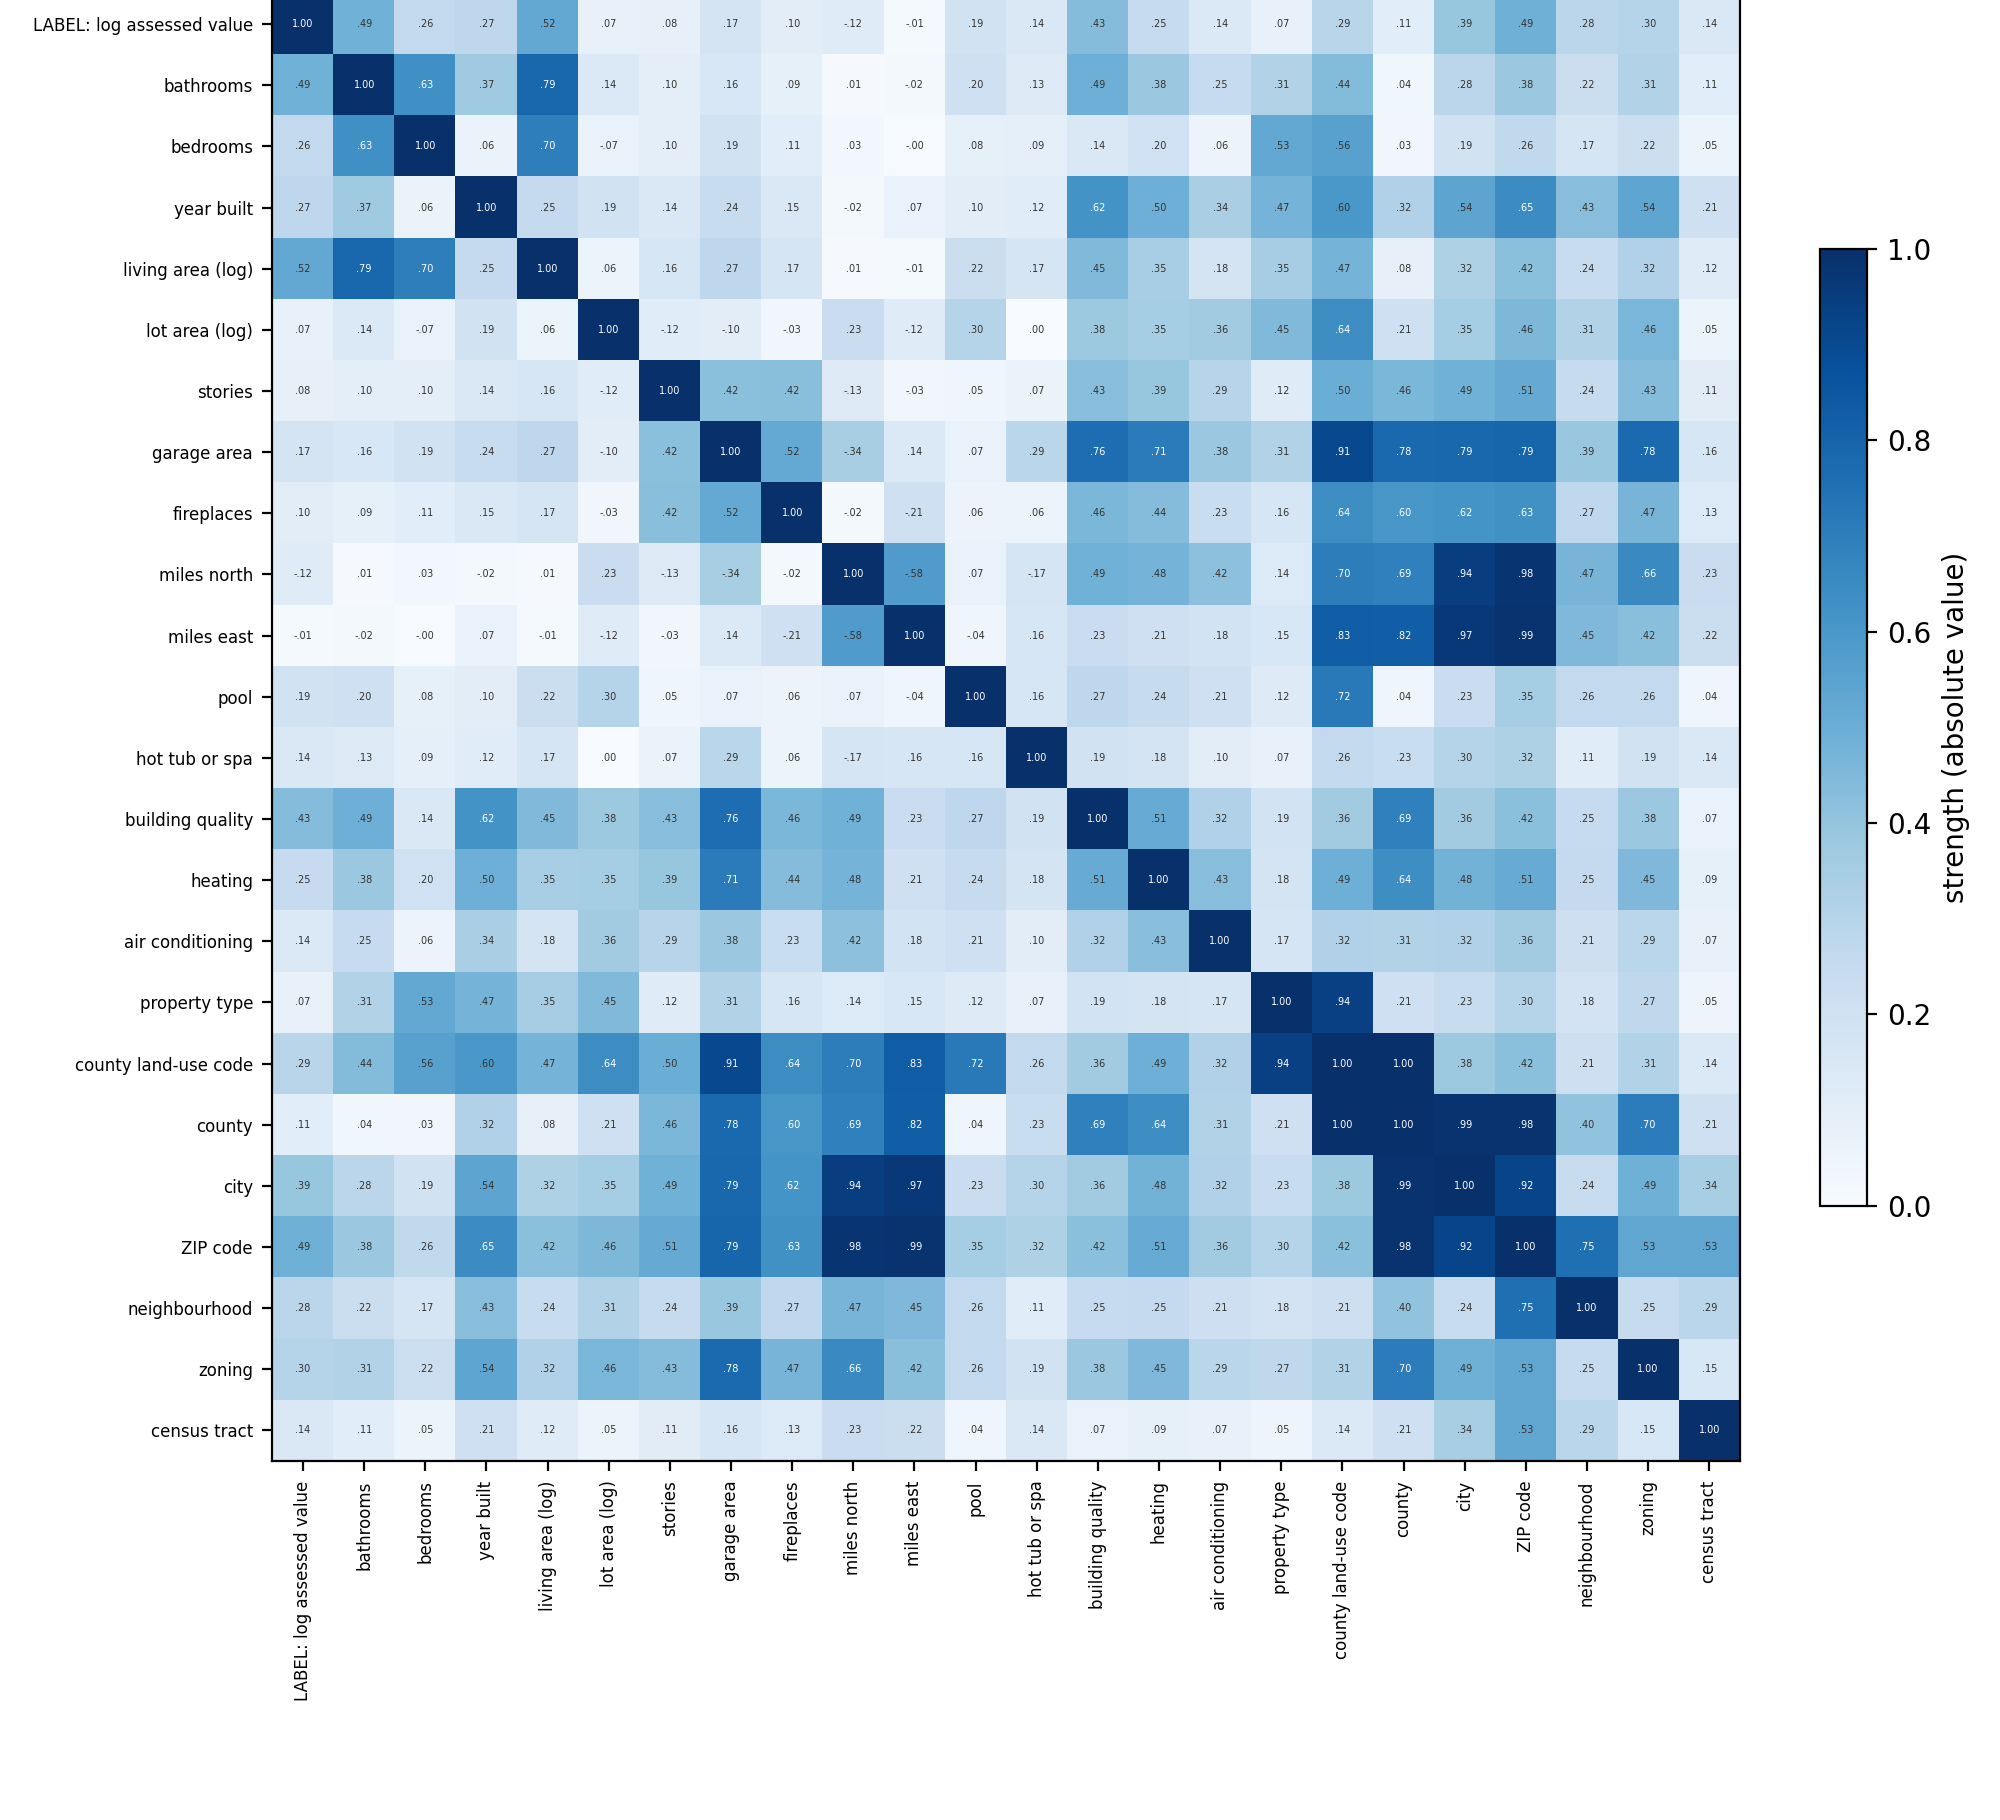
\includegraphics[width=0.78\textwidth]{figures/correlation_heatmap.png}
\caption{Association between the label and the 23 candidate features on the training homes: Pearson correlation for two numbers, correlation ratio on held-out homes for a category and a number, bias-corrected Cram\'er's V for two categories.}
\label{fig:heatmap}
\end{figure*}

\end{document}
